\section{Motivation}
\label{sec:intro:Motivation}

Realistic simulations involve complex relationships between an individual and the surroundings. Three types of interactions are possible whilst the individual performs complex decision making during an evacuation scenario. Through this thesis I aim to optimize these three types of interactions through various constraints and real time elements. The following encounters may be classified as below \cite{ref1}:

\begin{itemize}
  \item People-people interactions -  interactions between participating evacuees.
  \item People-structure interactions- interactions within the enclosed topology.
  \item People- environment interactions- interactions with quarantined atmosphere (fire, smoke etc.) and possible debris. 
\end{itemize}

During disaster scenarios standard evacuation pathways are often rigid and cannot autonomously provide modification for an exit strategy as the disaster ensues. The evacuees often find themselves in situations that force them to rely on general guidelines about how to react in emergency evacuation \cite{ref3}.  While such dynamic hazards cannot all be dealt with, using the traditional approach, Lujak, M., Billhardt H., Dunkel, J. et al \cite{ref4} attempts to help the evacuees adapt to the changing topography of the environment due to hazard dynamics by updating a real time monitoring system using an IoT architecture built in place within the premises of the said topology of the building. The above mentioned work uses a combination of IoT devices to sense and identify and provide real-time monitoring for the participating agents. Our work also obtains data from real time sources and then it is simulated with both macro and micro based agent models and then used to analyse and draw conclusions from the resulting data.

\section{Agent Based Model Simulation}
\label{sec:intro:Agent Based Model Simulation}

The present thesis is a design of a computational software using Agent Based Model (ABMS) to help speedy evacuation in emergency situations. Our software architecture help optimise the navigational flow rate in cases of real-time disaster management. The scenario is that of many victims are struck up in a very large building in the event of an occurrence of a disaster like fire, earthquake, poisonous chemical gas leakage, imminent bomb attack, potential imminent building collapse (similar to that of twin towers of 9/11). As a side benefit the experience acquired gives valuable information in the case of architecture design at the time of building construction itself. By conveying a suggestive path for each individual in the building at the time of disaster, the panic, erratic and groping movements are reduced to minimum helping to achieve a streamlined flow. Bottlenecks in the flow are avoided by redirecting people to alternate paths. The benefit of the overall perspective of the scenario and informed management is instantaneously conveyed to each and every individual in real time. The floor capacities and width of the doors and passageways form part of the constraints in the modelling. This is scalable and generic version.

\section{PedSim Simulator}
\label{sec:intro:PedSim Simulator}

PedSim is a pedestrian simulator tool designed as a front end to facilitate disaster management scenarios. Disaster management plans are multi-layered and topology specific. Tools catering to disaster management require the users to input topographic information and also provide crowd/agent location information. This aggregate of data is then processed initially to create a layout of the premises. The layout defines several rules and boundary conditions imposing restrictions for the crowd to navigate. Such information can be used to instantly model very specific scenarios such as evacuation of specific floors of a building. Since, PedSim enables input of design specific topology, protocols can be established quickly for speedy evacuation. The second part includes behaviour analysis of crowd during different disaster patterns. The social behaviour of victims in disaster afflicted scenarios have been of keen interest to researchers over the recent years. Disaster affected regions often portray victims who exhibit severe trauma or stress leading to emotional/psychological shut down or present themselves making erratic decisions etc. This tool enables a platform for crowd flow modelling. Erratic movement patterns can be modelled, simulated and visualized to study the impact and speed of evacuation. Such processed information can be used to provide instructions or navigation guidelines for optimal evacuation. PedSim also allows for real time monitoring of crowds providing instant feedback on the visual front end. This enables redirection of crowds for balancing congestion while developing exit strategies. Each exit can also be associated with restrictive exit capacity and corresponding flow rate ensuring crowd balancing.  The architectural design of the tool itself takes into account various factors such as streaming and batch processing of time critical data within permissible thresholds.

\section{Objectives and Approach}
\label{sec:intro:Objectives and Approach}

My work pertains to application of PedSim on our university building to implement and analyze the impacts of crowd evacuation during a disaster. The university building taken into consideration for our present study is level 3 of building (Coppito 0). The area under consideration is divided into 18 blocks. Each block consists of a set number of cells. Each cell represents a cubicle or a room. There are 26 cubicles/rooms in all. There is also one conference hall and two generic multipurpose areas used for allied purposes. In addition, there are several hallways and pathways for navigation. This area has four key exits distributed across the different boundary walls of the premises. At any given time, each cell hosts atmost twenty agents, reaching a maximum during peak hours of 10am to 2 pm Italy time. The premises often on average hosts about 100 people. We architected pedestrian flow simulations during a generic disaster which can include earthquake, fire and chemical leakage. The data is used to generate crowd clusters during events other than disasters such as workshops, cafeteria gatherings, conference gatherings etc. The figure \ref{clutter} shows a typical population cluster during a conference gathering. 

This thesis presents a case study where the Coppito 0 building is simulated during a disaster scenario using grid geometry based navigation algorithm as presented in the “An IoT Software Architecture for an Evacuable Building Architecture” by H.Muccini et.al \cite{ref5}. 

\begin{figure}[H]
  \centering
  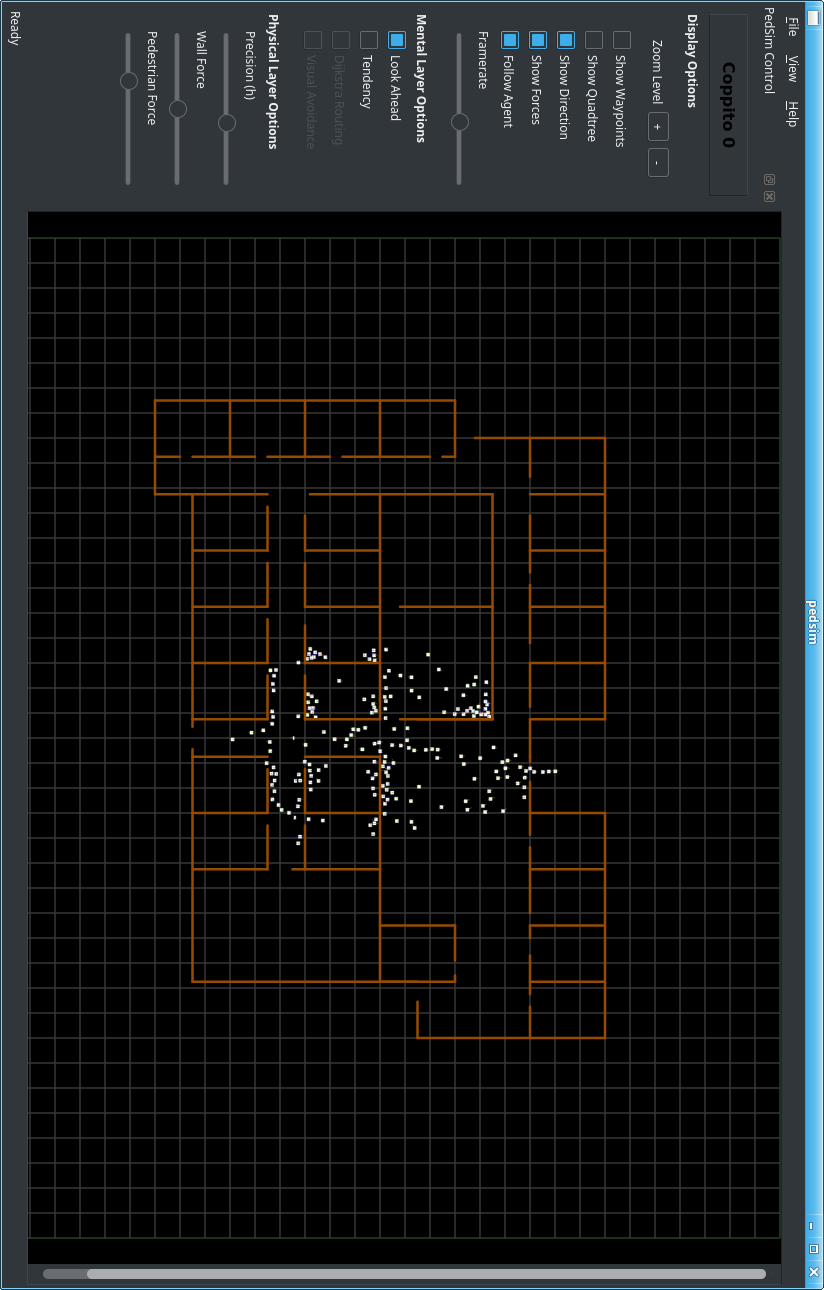
\includegraphics[scale=0.6]{implementation/clutter.png}
	\caption{Agent Cluster Formation in Coppito 0 Building}
  \label{clutter}
\end{figure}

The work also involves in expanding the capabilities of the existing PedSim simulation tool to include the new topology and the also to incorporate the algorithm and also further extended developed from the aforementioned paper and perform a real time analysis between micro and macro agents with the following criteria:

\begin{itemize}
  \item specifying the cells by social distances
  \item respecting the area capacity and doors capacities constraints
  \item varying movement speed according to various groups
  \item simulating social attachment among some agents 
\end{itemize}

As it is evident from the above constraints, the goal of this algorithm and this simulation is to make exit strategies as realistic as possible. By grouping certain agents together for instance, we can achieve realistic movement of participating agents, as in reality, people usually move in groups. families, friends etc. Furthermore, congestion is a big part of the evacuation scenario, as it is congestion that determines how fast or efficient the evacuation of agents occur and also how it would take to move groups of people. With groups of people clumped together, the next most natural constraint would be to assign varying speeds as not all agents and not all groups of agents travel with the same speed across the topology of the building. There is also one other constraint which determines the cell capacity, which determines how spaced out and occupied agents are in a room, a hall or a passageway. This also help determine how many can get through a single doorway in order to transition from one passageway to another. This of course leads to previously mentioned issue of congestion. 

All these constraints are hence taken into account as the simulation is performed in order to clock and test for the performance time and efficiency of the algorithm used for micro and macro model simulation.

\section{Thesis Outline}
\label{sec:intro:Thesis Outline}

The structure of the thesis is formulated as follows: chapter 2 provides a detailed literature and background work pertaining to the area of agent based simulation models and exit strategies. Chapter 3 focuses on the implementation details of the algorithm and specific scenario details that are incorporated in order to extend the algorithm in order to adapt it to a more realistic setting and also technical details regarding the PedSim simulation environment. Chapter 4 presents the results of the comparisons of the optimized(realistic) algorithm between the macro and micro agent simulation setting and to chart out the various performance metrics that are obtained. Chapter 5 attempts to draw conclusions based on the obtained performance metrics and also present the future work related to the aforementioned. This thesis also provides a technical appendix for reference for the simulation of various micro and macro agent scenarios within the environment of PedSim.